\section{Finding the Unsat Core}
With the aforementioned concepts and notations, we can formally state
the unsat core problem over polynomial rings as follows: 

\begin{Problem}
Let $F = \{f_1, \dots f_s\}$ be a set of multivariate polynomials in
the ring $R = \F[x_1,\dots,x_n]$ that generate ideal $J = \langle
f_1,\dots,f_s\rangle \subset R$. Suppose that it is known that $V(J) =
\emptyset$, or it is determined to be so by applying the Gr\"obner
basis algorithm. Identify a subset of polynomials $F_c \subseteq F,
J_c = \langle F_c \rangle$, such that $V(J_c) = \emptyset$
too. Borrowing the terminology from the Boolean SAT domain, we
call $F_c$ the infeasible core or the unsat core of $F$. 
\end{Problem}

Any set of polynomials $F$ with empty variety is an unsat core in
itself. There may be more than one unsat cores in $F$, some
polynomials may be common to multiple cores (i.e. the
cores may be non-disjoint), and these cores may have
different cardinalities $|F_c|$. The unsat core problems
are therefore further classified as: 
\bi
\item Identify a {\it minimum} core, i.e. a core of minimum
  cardinality. 
\item Identify a {\it minimal} core. An unsat core $F_{c}$ is minimal
  with respect to the property that while the variety of $F_{c}$ is
  empty, the variety of {\it any} subset of $F_c$ is {\it non-empty},
  i.e. $V( F_{c} - \{f_i\} ) \neq \emptyset$ for any $f_i \in
  F_c$. 
\item Identify any unsat core disregarding minimality; i.e. find any
  subset $F_c$ of $F$.
\ei

Let us first consider the problem of finding any $F_c \subset F$,
disregarding minimality. It is not hard to motivate that an unsat
core should be identifiable using the Gr\"obner basis
algorithm: Assume that $F_c = F - \{f_j\}$. If $GB(F) = GB(F_c) =
\{1\}$, then it implies that $f_j \in \langle F - \{f_j\}\rangle$. In
other words, 
$f_j$ can be composed of the other polynomials of $F_c$, so $f_j$ is
not a part of the unsat core, and it can be safely discarded from
$F_c$. This can be identified by means of the GB algorithm for this
ideal membership test (due to Def. \ref{def:gb}(ii)). 

A n\"aive way (and inefficient way) to identify {\it a minimal core}
using the GB computation is as follows:
selectr a polynomial $f_i$ and see if $V(F_c - \{f_i\}) = \emptyset$
(i.e. if reduced $GB(F_c - \{f_i\}) = \{1\}$). If so, discard $f_i$
from the core; otherwise retain $f_i$ in $F_c$. Select a different
$f_i$ and continue until all polynomials $f_i$ are visited for
inclusion in $F_c$. This approach will produce a minimal core, as we
would have tested each polynomial $f_i$ for inclusion in the
core. This requires $O(|F|)$ calls to the GB engine, which is really
impractical.   

\subsection{Investigating algorithmic techniques to find $F_c$ from $F$}

We investigate if it is possible to identify a core by analyzing the
$Spoly(f_i,f_j)\xrightarrow{F}_+ r$ reductions in Buchberger's
algorithm. Since $F$ is an unsat core, 
definitely {\it there exists  
a sequence of Spoly reductions in Buchberger's algorithm where
$Spoly(f_i, f_j) \xrightarrow{F}_+ 1$ is achieved.} Moreover, 
polynomial reduction algorithms can be suitably modified to record
which polynomials from $F$ are used in the division leading to
$Spoly(f_i,f_j)\xrightarrow{F}_+1$. This suggests that by recording
the {\it ``data''} generated by Buchberger's algorithm --- i.e. the
critical pair polynomials ($f_i,f_j$) used in the Spoly computations,
and the polynomials from $F$ used to cancel terms in the reduction
$Spoly(f_i,f_j)\xrightarrow{F}_+1$ --- we should be able to identify a
core. 

We will use an example to demonstrate our approach of identifying $F_c
\subseteq F$ using this ``data'':

\begin{example}
\label{ex:1}
Consider the following set of polynomials:
\begin{center}
$f_1: abc + ab + ac + bc + a + b + c + 1$
\end{center}
\begin{center}
$f_2: b$
\end{center}
\begin{center}
$f_3: ac$
\end{center}
\begin{center}
$f_4: ac + a$
\end{center}
\begin{center}
$f_5: bc + c$
\end{center}
\begin{center}
$f_6: abd + ad + bd + d$
\end{center}
%\newpage
\begin{center}
$f_7: cd$
\end{center}
\begin{center}
$f_8: abd + ab + ad + bd + a + b + d + 1$
\end{center}
\begin{center}
$f_9: abd + ab +bd + b$
\end{center}

Assume $>_{DEGLEX}$ monomial ordering with $a>b>c>d$. 
Let $F = \{f_1,\dots,f_9\}$ and 
$J = \langle F \rangle \subset \mathbb{F}_2[a,b,c,d]$ where
$\mathbb{F}_2 = \{0, 1\}$ is the finite field of 2 elements. Then 
$V(J) = \emptyset$ as $GB(J) = 1$.  The set $F$ consists of 4 {\it minimal}
cores: $F_{c1} = \{ f_1,f_2,f_3,f_4,f_7,f_8\}, F_{c2} = \{
f_2,f_4,f_5,f_6,f_8\}, F_{c3} = \{ f_2,f_3,f_4,f_6,f_8\},$ and $F_{c4}
= \{ f_1,f_2,f_4,f_5\}$. 
\end{example}

Buchberger's algorithm terminates to a unique reduced GB, irrespective
of the order in which the critical pairs are selected and reduced as
$Spoly(f_i,f_j)\xrightarrow{F}_+r$. Let us suppose that in the GB
computation corresponding to Example \ref{ex:1}, the first 3 critical
pairs analyzed are $(f_1, f_2), (f_3, f_4)$ and $(f_2,f_5)$. It turns
out that the Spoly-reductions corresponding to these 3 pairs lead to
the unit ideal. Recording the ``data'' corresponding to this sequence
of reductions is depicted in Fig. \ref{fig:refute}. We call this
graph a refutation tree. 


\begin{figure}[hbt]
\centering
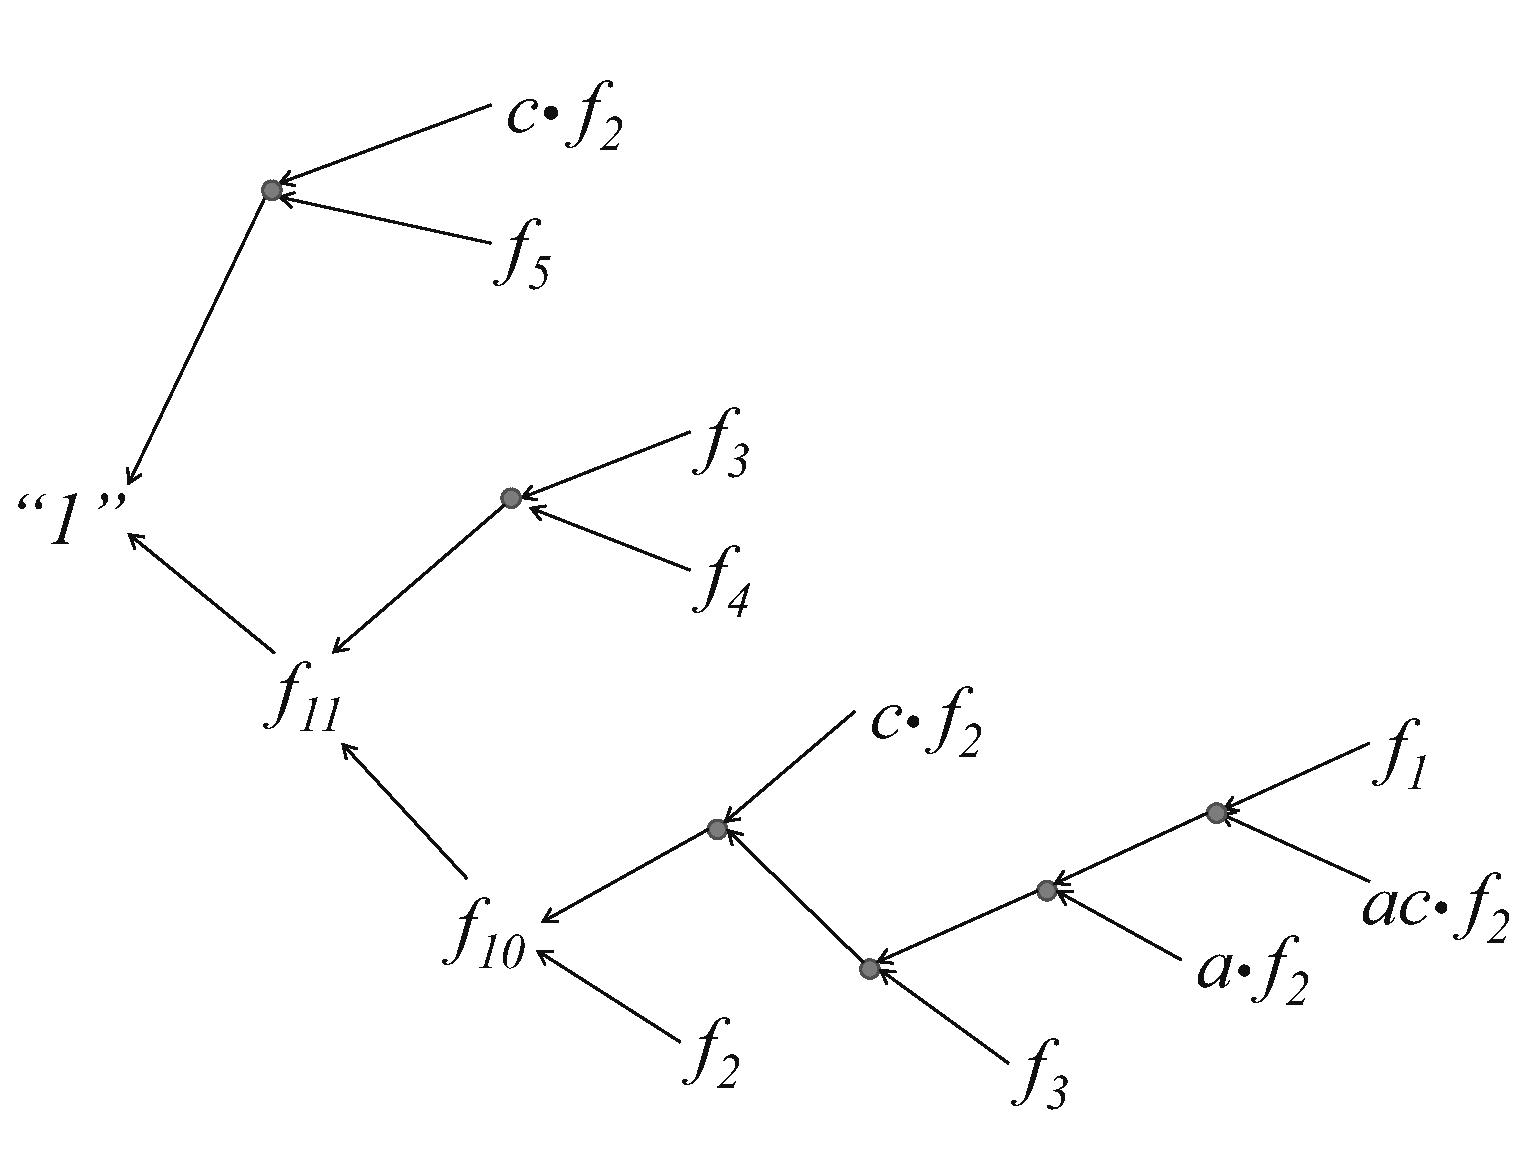
\includegraphics[scale=0.25]{./SAT2016_xiaojun/refutation_tree.eps}
\caption{Generating refutation trees to record unsat cores.}
\label{fig:refute}
\end{figure}

In the figure, the nodes of the graph correspond to the polynomials
utilized in Buchberger's algorithm. The leaf nodes always correspond
to polynomials $f_i \in F$. An edge $e_{ij}$ from node $i$ to node $j$
signifies that the polynomial at node $j$ resulted from polynomial
$i$. For example, consider the computation
$Spoly(f_1,f_2)\xrightarrow{F}_+ f_{10}$, where $f_{10} = a + c +
1$. Since $Spoly(f_1, f_2) = f_1 - ac\cdot f_2$, the leaves
corresponding to $f_1$ and $ac\cdot f_2$ are created. The reduction
$Spoly(f_1,f_2)\xrightarrow{F}_+ f_{10}$ is carried out as the
following sequence of 1-step divisions:
$Spoly(f_1,f_2)\xrightarrow{a\cdot f_2} \xrightarrow{f_3}
\xrightarrow{c\cdot f_2}  \xrightarrow{f_2} f_{10}$. This is depicted
as the bottom subtree in the figure, terminating at polynomial
$f_{10}$. Moreover, the multiplication $a\cdot f_2$ implies that
division by $f_2$ resulted in the quotient $a$. The refutation tree of
Fig. \ref{fig:refute} shows further that
$Spoly(f_3,f_4)\xrightarrow{f_{10}} f_{11} = c+1$ and, finally,
$Spoly(f_5,f_2)\xrightarrow{f_{11}} 1$. 
 
To identify an $F_c \subset F$, we start from the refutation node
$''1''$, and traverse the graph in reverse, all the way upto the
leaves. Then, all the leaves in the transitive fanin of ``1''
constitute an unsat core. The polynomials (nodes) that do not lie in
the transitive fanin of ``1'' can be safely discarded from $F_c$. From
Fig. \ref{fig:refute}, $F_c = \{f_1,f_2,f_3,f_4,f_5\}$ is identified
as an unsat core of $F$. 

\subsubsection{Ordering critical pairs in Buchberger's algorithm:} It
is clear that the inclusion of polynomials in the obtained core
depends on the order in which the critical pairs are
reduced. This is a well-known intractable problem, and various
heurstics have been proposed to favourably influence the termination
of the Gr\"obner basis algorithm -- these include the sugar
strategy \cite{GBSelectionStrategies}, the preconditioning used by
{\it Faug\~{e}re} in the $F4$ algorithm \cite{f4}, among others. Any
such selection strategy can be also be applied in our setting to
identify a smaller core. 

\section{Reducing the Size of the Infeasible Core $F_c$}

The core $F_c$ obtained from the aforementioned procedure is not
guaranteed to be minimal. For example, let us revisit the the core
$F_c=\{f_1,\dots, f_5\}$ generated in the previous section. Note that
while $F_c$ is a smaller infeasible core of $F$, it is not minimal. In
fact, Example 1 shows that $F_{c4} =\{f_1,f_2,f_4,f_5\}$ is the
minimal core where $F_{c4} \subset F_{c}$. Clearly, the polynomial
$f_3 \in F_c$ is a redundant element of the core. It could be
discarded. We will now describe how the size of this core could be
reduced further.  For this purpose, we will have to perform a more
systematic book-keeping of the data generated during the execution of
Buchberger's algorithm and the refutation tree. 

\subsection{Identifying redundant polynomials from the refutation tree}

We will keep track of the S-polynomials that give a non-zero remainder
when divided by the system of polynomials $F$ at that moment:
\begin{equation}
\label{eqn1}
g_{ij}= S(f_i,f_j)+\displaystyle\sum_{k=1}^m c_kf_k,
\end{equation}
where $0\neq c_k\in\mathbb{F}[x_1,\ldots,x_n]$ and
$\{f_1,\ldots,f_l\}$ is the ``current'' system of polynomials
$F$. For each non-zero $g_{ij}$, we will record the following data: 

\begin{equation}
\label{data1}
((g_{ij})(f_{i},h_{ij})(f_{j},h_{ji})| (c_{k1},f_{k1}),(c_{k2},f_{k2}),\dots,(c_{kl},f_{kl}))
\end{equation}

Note that in (\ref{eqn1}) and (\ref{data1}), $g_{ij}$ denotes the
remainder of the $S$-polynomial $S(f_i,f_j)$ modulo the current system
of polynomials $f_1,\ldots,f_m$, and we denote by  

$$h_{ij}:=\displaystyle\frac{\lcm(lm(f_i),lm(f_j))}{lt(f_i)},
h_{ji}:=\displaystyle\frac{\lcm(lm(f_i),lm(f_j))}{lt(f_j)}$$ 
the coefficients of $f_i$, respectively $f_j$, in the $S$-polynomial
$S(f_i,f_j)$. Furthermore, in (\ref{data1}), $(c_{k1}, \dots c_{kl})$ are the
polynomial coefficients of $(f_{k1}, \dots,f_{kl})$ that appear in the
division process. 

\begin{example}
Revisiting Example \ref{ex:1},  the data corresponding to
$Spoly(f_1,f_2)\xrightarrow{F}_+  g_{12} = f_{10}$ reduction is
obtained as the following sequence of computations:
$$f_{10}=g_{12}=f_1-acf_2-af_2-f_3-cf_2-f_2.$$ As the coefficient
field is $\mathbb{F}_2$ in this example, $-1 = +1$, so:
$$f_{10}=g_{12}=f_1+acf_2+af_2+f_3+cf_2+f_2$$ is obtained.
The data is recorded according to (\ref{data1}):

\begin{center}
$((f_{10}=g_{12}), (f_1,1)(f_2,ac)|(a,f_2),(1,f_3),(c,f_2),(1,f_2))$
\end{center}

\end{example}

Of course, our approach and the book-keeping stops when we obtain
1 as the remainder of the S-polynomial modulo the current system of
generators. As an output of the Buchberger's algorithm, we can obtain
not only the Gr\"obner bases,  $G = \{g_1,\ldots,g_t\}$, but also a
matrix $M$ such that: 
\begin{center}
\begin{align}
   \begin{bmatrix}
           g_{1} \\
           g_{2} \\
           \vdots \\
           g_{t}
         \end{bmatrix}
    &= M \begin{bmatrix}
           f_{1} \\
           f_{2} \\
           \vdots \\
           f_{s}
         \end{bmatrix}
  \end{align}

\end{center}

Each element $g_i$ of $G$ is a polynomial combination of $f_1, \dots,
f_s\}$. Moreover, this matrix $M$ is constructed precisely using the
data that is recorded in the form of (\ref{data1}). We now a condition
when the matrix $M$ may identify some redundant elements. 


\begin{theorem}
\label{thm}
With the notations above, we have that a core for the system of
generators $F = \{f_1,\dots,f_s\}$ of the ideal $J$ is given by the
union of those $f_i$'s from $F$ that appear in the data recorded above
and correspond to the nonzero entries in the matrix $M$.  
\end{theorem}

\begin{proof}
In our case, since the variety is empty, and hence the ideal is the
unit ideal, we have that $G = \{g_1=1\}$ and $t=1$. Therefore $M=
[a_1, \ldots, a_s]$ is a vector. Then the output of the algorithm
gives:

$$1 = a_1f_1+\cdots + a_s f_s.$$ Clearly, if $a_i=0$ for some $i$ then
$f_i$ does not appear in this equation and should not be included in
the infeasible core of $F$. 

\end{proof}


\begin{example}

Corresponding to Example \ref{ex:1} and the refutation tree shown in
Fig. \ref{fig:refute}, we discover that the polynomial $f_3$ is used
only twice in the division process. In both occasions, the quotient of
the division is 1. Therefore, from Fig. \ref{fig:refute}, it follows that:
\begin{equation}
1 = (f_2 + f_5) + \dots + \mathbf{1\cdot f_3} + \dots + \mathbf{1\cdot f_3}+ \dots (f_1
+ f_2)
\end{equation}

Since $1 + 1 = 0$ over $\F_2$, we have that the entry in $M$
corresponding to $f_3$ is 0, and so $f_3$ can be discarded from the
core. 
\end{example}

\subsection{The GB-Core Algorithm Outline}

The following steps describe an algorithm (GB-Core) that allows us to compute a
refutation tree of the polynomial set and corresponding matrix $M$. 

{\bf Inputs:} Given a system of polynomials $F=\{f_1,\ldots,f_s\}$
, a monomial order $>$ on $\mathbb{F}[x_1,\ldots,x_n]$. 

{\bf S-polynomial reduction:} We start computing the S-polynomials of the system of
generators $\{f_1,\ldots,f_s\}$, then divide each of them by the system of
generators $G=\{f_1,\dots,f_s,\dots,f_m\}$ which is the intermediate result of Buchberger's algorithm. 
In this way, we obtain the following expression:
\begin{equation}
\label{eqn:red}
g_{ij}= h_{ij}f_{i}+h_{ji}f_{j}+\displaystyle\sum_{k=1}^m c_kf_k
\end{equation}
If the remainder $g_{ij}$ is non-zero, we will denote it by
$f_{m+1}$ and we will add it to intermediate system of generators $G$. We
will also record the data as (\ref{data1}): 
\begin{displaymath}
((f_{m+1}=g_{ij})(f_{i},h_{ij})(f_{j},h_{ji})| (c_{k1},f_{k1}),(c_{k2},f_{k2}),\dots,(c_{kl},f_{kl}))
\end{displaymath}
It forms a tree with root $f_{m+1}$.

{\bf Coefficients recording:} In (\ref{eqn:red}) we get a coefficient vector including coefficients
$c_k$ where $k>s$. These coefficients are associated with new generators in the Gr\"obner basis,
which cannot benefit the UNSAT core extraction. Therefore we need to rewrite the vector to
one with only $c_k, k=1\dots s$, which can be achieved by substituting $f_k,k>s$ by $f_1,\dots,f_s$:
initially we have $f_{s+1}= c_1f_1 + c_2f_2 + \cdots + (h_{ij}+c_i)f_{i}+\cdots+(h_{ji}+c_j)f_{j}+\cdots+c_sf_s$,
inductively if we can present $f_{s+1}$ to $f_{s+k-1}$ by $f_1,\dots,f_s$, we can also rewrite
$f_{s+k} = d_1f_1+\cdots+d_sf_s$. Then we add a new row $ (d_1,\dots,d_s ) $ to coefficient matrix $M$.

{\bf Termination and refutation tree construction:} By repeating S-polynomial reduction and coefficients 
recording until we get remainder $f_m = 1$, the algorithm
will generate a set of new generators $G$ and coefficient matrix $M$.
Meanwhile we can construct the refutation tree with the recorded data.
We start with 
\begin{displaymath}
((f_{m}=1)(f_{i},h_{ij})(f_{j},h_{ji})| (c_{k1},f_{k1}),(c_{k2},f_{k2}),\dots,(c_{kl},f_{kl}))
\end{displaymath}
It represents a tree start from leaves $f_{i}, f_j$ then internal nodes $f_{k1},\dots,f_{kl}$
and ``1" as the root. Next we substitute nodes $f_{m-1}, f_{m-2}, \dots, f_{s+1}$ in order
with corresponding subtrees. The algorithm returns the complete refutation tree as well as
matrix $M$.

The complete algorithm is concluded as pseudo code below:

\begin{algorithm}[H]
 \caption{GB-core algorithm (based on Buchberger's algorithm)}
 \label{algo:gbcore}
 \begin{algorithmic}[1]

 \REQUIRE $F = \{f_1, \dots, f_s\} \in \F[x_1, \dots, x_n], f_i\neq 0$
 \ENSURE Refutation tree $T$ and coefficients matrix $M$
 \STATE{ {Initialize: list $G \gets F$; Dataset $D\gets \emptyset$; $M\gets s\times s$ unit matrix} }
 \FOR {{ each pair $(f_i,f_j)\in G$  }}
 	\STATE  $f_{sp},(f_{i},h_{ij})(f_{j},h_{ji}) \gets$ spoly-pair($f_i,f_j$) \COMMENT{$f_{sp}$ is the S-polynomial}
 	\STATE{{ $g_{ij}|(c_{k1},f_{k1}),\dots,(c_{kl},f_{kl}) \gets (sp\xrightarrow{G}_+  g_{ij})$}}
 	\IF{{ $g_{ij} \neq 0$ }}
 		\STATE {{$G \gets G \cup g_{ij}$}}
 		\STATE {{Update $D$ and $M$}}
 	\ENDIF
 	\IF {{$g_{ij} = 1$}}
 		\STATE {{Construct $T$ from $D$}}
 		\STATE {{ Return($T,M$) }}
 	\ENDIF
 \ENDFOR
 \end{algorithmic}
 \end{algorithm}



\section{Iterative Refinement of the Unsat Core}
Similar to all other core extractors, our algorithm cannot generate a
minimal core in one execution. To obtain a smaller core, we need to
re-execute our tool with the core obtained in the current
iteration. We describe two heuristics that are applied to our
algorithm to increase the probability to generate a smaller core in
the next iteration. 

After eliminating all redundant polynomials, we can call our GB engine
with the new core. A effective heuristic should enhance the
probability that the refutation "1" is composed by fewer polynomials. 
In our GB computing algorithm, we use a strategy to pick critical
pairs such that polynomials with  larger indexes get involved as late
as possible: 
$$(f_1,f_2)\to(f_1,f_3)\to(f_2,f_3)\to(f_1,f_4)\to(f_2,f_4)\to\cdots$$

Meanwhile, for the reduction process $Spoly(f_i,f_j)\xrightarrow{F}_+
f_{new}$, we pick divisor polynomials from $F$ following the order of
polynomial indexes. Therefore, by renaming the polynomial indexes, we
can increase the likelihood they are selected into the unsat core. 
We use 2 criteria to increase the probability that a polynomial is
included in the refutation tree.  One corresponds to the \emph{refutation distance},
whereas the other corresponds to the frequency that
a polynomial appears in refutation tree. 

\begin{definition}
\emph{Refutation distance} in a refutation tree corresponds to the number of arcs on
the shortest path from refutation "1" to a leaf
polynomial.
\end{definition}

Polynomials with shorter refutation distance are used as
divisors in later stages of polynomial reductions, which indicates
they will generally have lower degree leading terms.  
This is because we are assuming a degree-lexicographic order, and
successive term cancellations reduce the degree of the remainders. So
polynomials with lower degree leading terms are more  likely to be
used for reduction, such that the probability that they appear in
the refutation tree is larger.  

Similarly, the motivation for \emph{frequency of appearance} of $f_i$ in
the refutation tree is as follows: polynomials appearing frequently in
the refutation tree also indicates that they have some properties
(leading terms) that make them "favourable" in the unsat core
selection. For example, their leading terms may contain variables
that are require them to be included in the minimal core. 

We apply both heuristics: we sort the polynomials in the core
by the refutation distance criterion, and use the frequency criterion as
the tiebreaker. The following example illustrates our heuristic. 


%\vspace{5mm}\\
\begin{example} 
Consider a set of 6 polynomials over $\F_2$ of an
infeasible instance.
\begin{align*}
f_1 &: x_1x_3+x_3\\
f_2 &: x_2 + 1\\
f_3 &: x_2x_3+x_2\\
f_4 &: x_2x_3\\
f_5 &: x_2x_3 + x_2 + x_3 + 1\\
f_6 &: x_1x_2x_3 +x_1x_3
\end{align*}

After the first iteration, we get a tree of refutation as shown in Fig.\ref{fig:refine}(a). 
\begin{figure}[hbt]
\centering
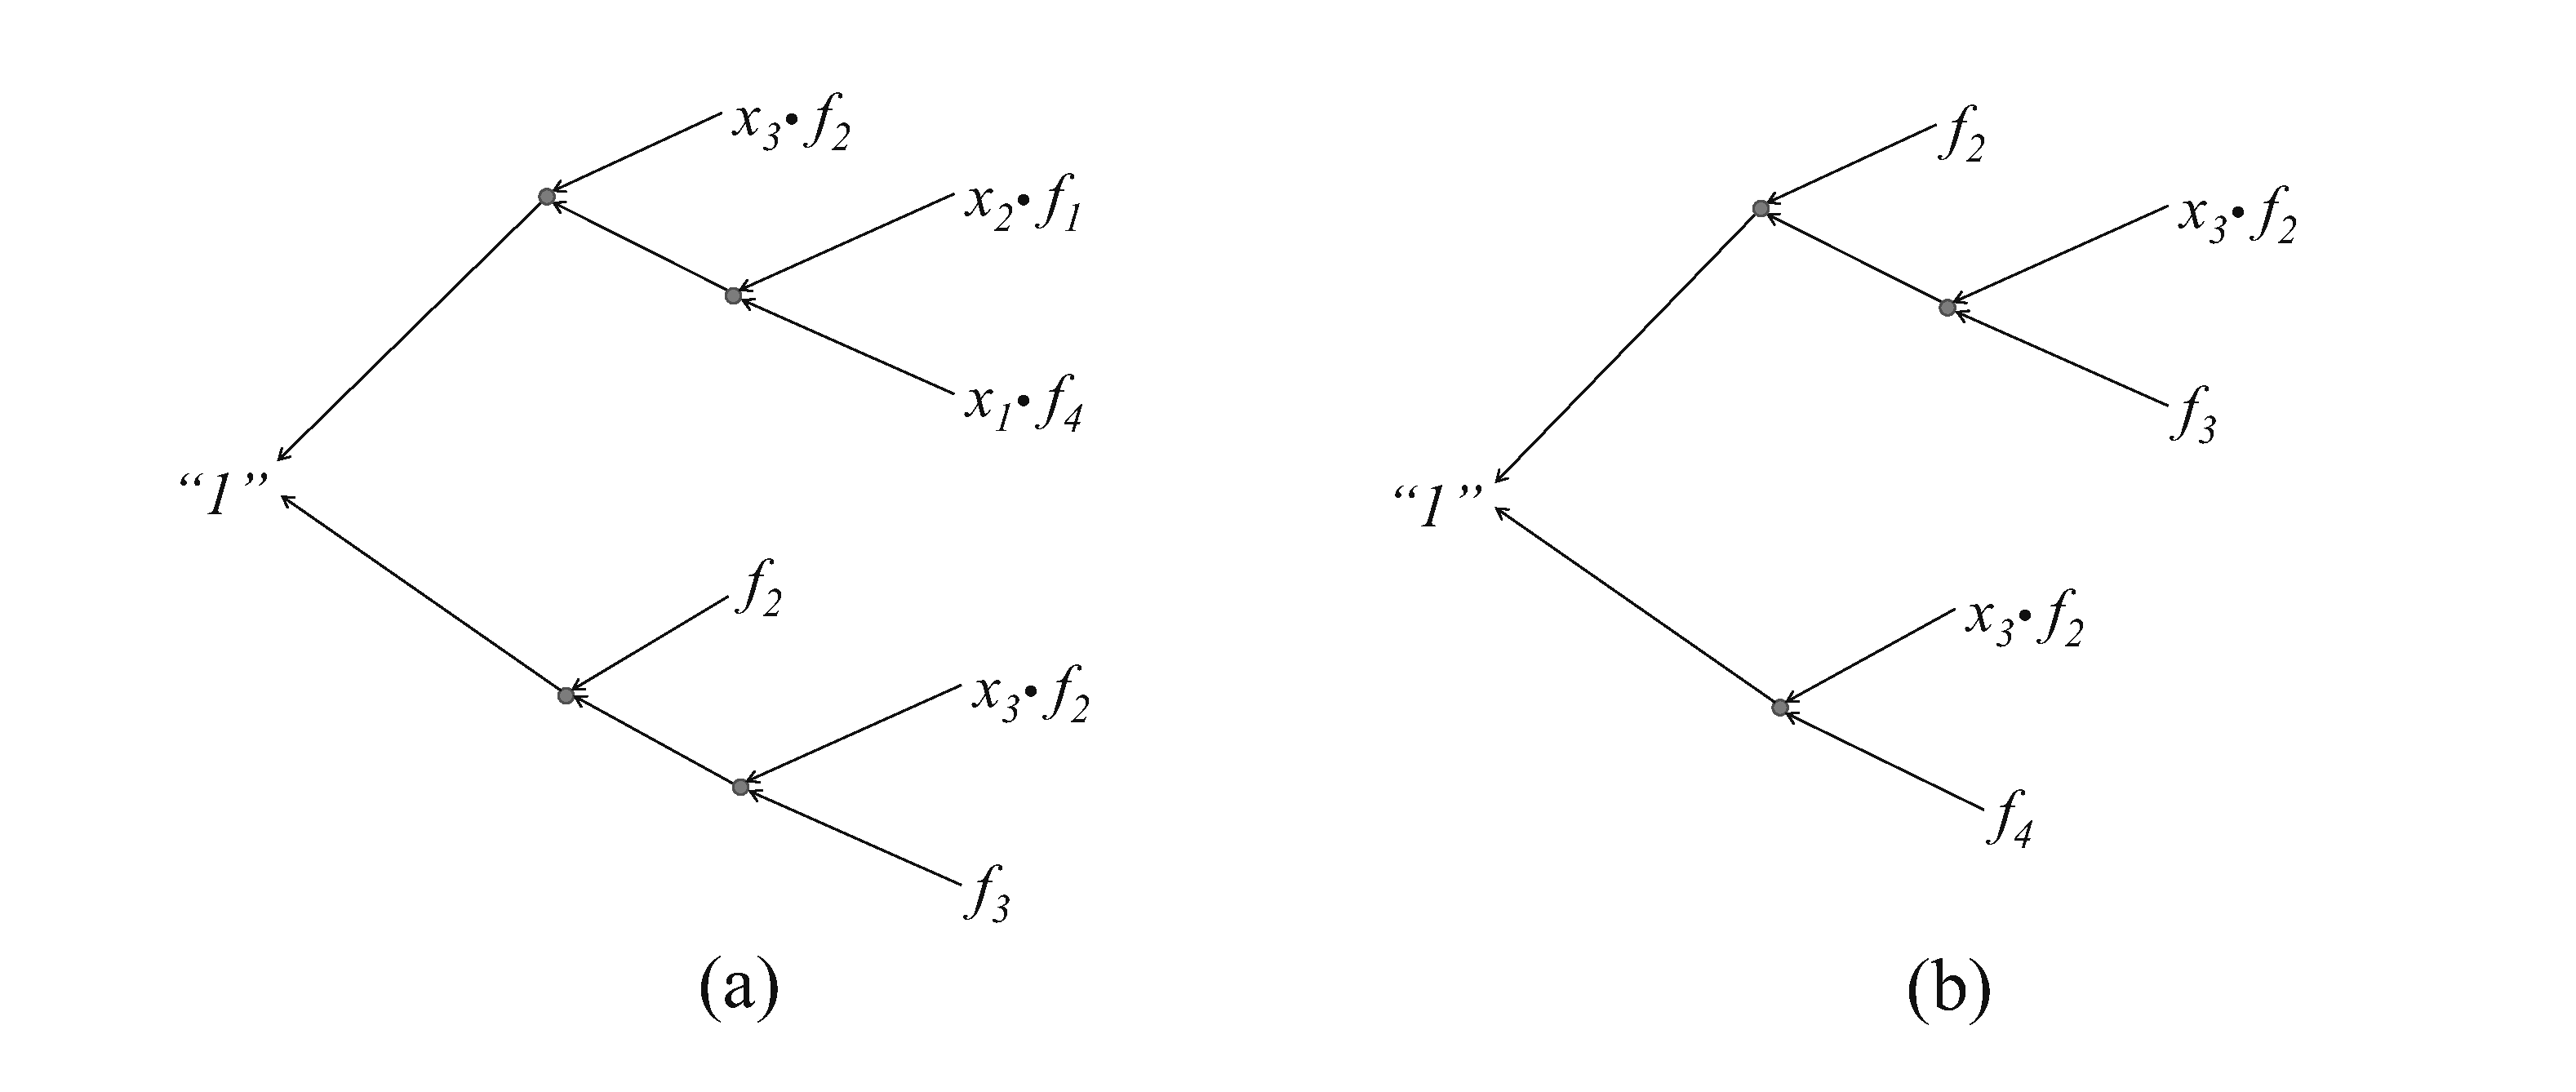
\includegraphics[scale=0.25]{SAT2016_xiaojun/core_refine.eps}
\caption{Refutation trees of core refinement example}
\label{fig:refine}
\end{figure}

The shortest "Distance" corresponds to that of $f_2$ to "1", which is
2 levels. So, we reorder $f_2$ to be the polynomial with the shortest
index. The "distance" and "frequency" for other polynomials are
identical, so we keep their ordering untouched. We re-index the
polynomial set 
$$f_1'=f_2, f_2' = f_1, f_3' = f_3, f_4' = f_4$$
and apply our GB-core algorithm on $\{f_1',f_2',f_3',f_4'\}$. The
result is shown in Fig.\ref{fig:refine}(b). We reach a fixpoint, and
the core $\{f_1', f_3', f_4'\} = \{f_2,f_3,f_4\}$ is proved to be
minimal. 
\end{example}
